\documentclass[notes,serif]{beamer}
\usepackage{graphicx}
\usepackage{url}
\usepackage{clrscode}
\usepackage{amssymb,amsmath}

% You should run 'pdflatex' TWICE, because of TOC issues.

\mode<presentation>
{
  % A tip: pick a theme you like first, and THEN modify the color theme, and then add math content.
  % Warsaw is the theme selected by default in Beamer's installation sample files.

  %%%%%%%%%%%%%%%%%%%%%%%%%%%% THEME
  %\usetheme{AnnArbor}
  %\usetheme{Antibes}
  %\usetheme{Bergen}
  %\usetheme{Berkeley}
  %\usetheme{Berlin}
  %\usetheme{Boadilla}
  %\usetheme{boxes}
  %\usetheme{CambridgeUS}
  %\usetheme{Copenhagen}
  %\usetheme{Darmstadt}
  %\usetheme{default}
  %\usetheme{Dresden}
  %\usetheme{Frankfurt}
  %\usetheme{Goettingen}
  %\usetheme{Hannover}
  %\usetheme{Ilmenau}
  %\usetheme{JuanLesPins}
  %\usetheme{Luebeck}
  %\usetheme{Madrid}
  %\usetheme{Malmoe}
  %\usetheme{Marburg}
  %\usetheme{Montpellier}
  %\usetheme{PaloAlto}
  %\usetheme{Pittsburgh}
  %\usetheme{Rochester}
  %\usetheme{Singapore}
  %\usetheme{Szeged}
  \usetheme{Warsaw}

  %%%%%%%%%%%%%%%%%%%%%%%%%%%% COLOR THEME
  %\usecolortheme{albatross}
  %\usecolortheme{beetle}
  %\usecolortheme{crane}
  \usecolortheme{default}
  %\usecolortheme{dolphin}
  %\usecolortheme{dove}
  %\usecolortheme{fly}
  %\usecolortheme{lily}
  %\usecolortheme{orchid}
  %\usecolortheme{rose}
  %\usecolortheme{seagull}
  %\usecolortheme{seahorse}
  %\usecolortheme{sidebartab}
  %\usecolortheme{structure}
  %\usecolortheme{whale}

  %%%%%%%%%%%%%%%%%%%%%%%%%%%% OUTER THEME
  %\useoutertheme{default}
  %\useoutertheme{infolines}
  %\useoutertheme{miniframes}
  %\useoutertheme{shadow}
  %\useoutertheme{sidebar}
  %\useoutertheme{smoothbars}
  %\useoutertheme{smoothtree}
  %\useoutertheme{split}
  %\useoutertheme{tree}

  %%%%%%%%%%%%%%%%%%%%%%%%%%%% INNER THEME
  %\useinnertheme{circles}
  %\useinnertheme{default}
  %\useinnertheme{inmargin}
  %\useinnertheme{rectangles}
  %\useinnertheme{rounded}

  %%%%%%%%%%%%%%%%%%%%%%%%%%%%%%%%%%%

%  \setbeamercovered{transparent} % or whatever (possibly just delete it)
  \setbeamercovered{invisible} % or whatever (possibly just delete it)
  % To change behavior of \uncover from graying out to totally invisible, can change \setbeamercovered to invisible instead of transparent. apparently there are also 'dynamic' modes that make the amount of graying depend on how long it'll take until the thing is uncovered.

}


% Get rid of nav bar
\beamertemplatenavigationsymbolsempty

% Use short top
%\usepackage[headheight=12pt,footheight=12pt]{beamerthemeboxes}
%\addheadboxtemplate{\color{black}}{
%\hskip0.3cm
%\color{white}
%\insertshortauthor \ \ \ \
%\insertframenumber \ \ \ \ \ \ \
%\insertsection \ \ \ \ \ \ \ \ \ \ \ \ \ \ \ \ \  \insertsubsection
%\hskip0.3cm}
%\addheadboxtemplate{\color{black}}{
%\color{white}
%\ \ \ \
%\insertsection
%}
%\addheadboxtemplate{\color{black}}{
%\color{white}
%\ \ \ \
%\insertsubsection
%}

% Insert frame number at bottom of the page.
\usefoottemplate{\hfil\tiny{\color{black!90}\insertframenumber}}

\usepackage[english]{babel}
\usepackage[latin1]{inputenc}

\usepackage{times}
\usepackage[T1]{fontenc}

\title{Design and Analysis of Algorithms}
\subtitle{Lecture 6---Binary Search Trees}

\author{Lei Wang}

\institute{Dalian University of Technology}

%\date{Date}
\date{October 8, 2008}

\subject{Talks}

\def\defn#1{{\color{red} #1}}

\begin{document}

\begin{frame}
  \titlepage
\end{frame}

\begin{frame}
  \frametitle{Binary Search Trees}
  \tableofcontents
\end{frame}

\section{Overview}
\subsection{Goals}

\begin{frame}
\frametitle{Goals}
\begin{itemize}
    \item Binary search trees, tree walks, and operations on binary search trees.
\end{itemize}
\end{frame}

\section{Search Trees}

\subsection{Search trees}

\begin{frame}
  \frametitle{Search Trees}
    \begin{itemize}
      \item Data structures that support many dynamic-set operations.
      \item Can be used as both a dictionary and as a priority queue.
      \item Basic operations take time proportional to the {\bf\em height} of the tree.
      \item For complete binary tree with $n$ nodes: worst case $\Theta(\text{lg}n)$.
      \item For linear chain of $n$ nodes: worst case $\Theta(n)$.
      \item Different types of search trees include binary search trees, red-black trees
(covered in Chapter 13), and B-trees (covered in Chapter 18).
    \end{itemize}
\end{frame}

\section{Binary Search Trees}
\begin{frame}
  \frametitle{Binary search trees}
  Binary search trees are an important data structure for dynamic sets.
  \begin{itemize}
    \item Accomplish many dynamic-set operations in $O(h)$ time, where $h$ = height of
tree.
    \item Each node contains the fields
    \begin{itemize}
      \item $key$ (and possibly other satellite data).
      \item $left$: points to left child.
      \item $right$: points to right child.
      \item $p$: points to parent. $p[root[T ]] = \textsc{nil}$.
    \end{itemize}
    \item Stored keys must satisfy the {\bf \em binary-search-tree} property.
    \begin{itemize}
      \item If $y$ is in left subtree of $x$, then $key[y]  \leq key[x]$.
      \item If $y$ is in right subtree of $x$, then $key[y] \ge key[x]$.
    \end{itemize}
  \end{itemize}
%  \begin{block}{\textsc{Hire-Assistant($n$)}}
%    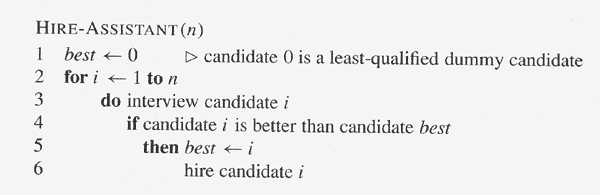
\includegraphics[height=3.5cm]{05-hire_assistant}
%  \end{block}
\end{frame}

\begin{frame}
  \begin{block}{Example}
    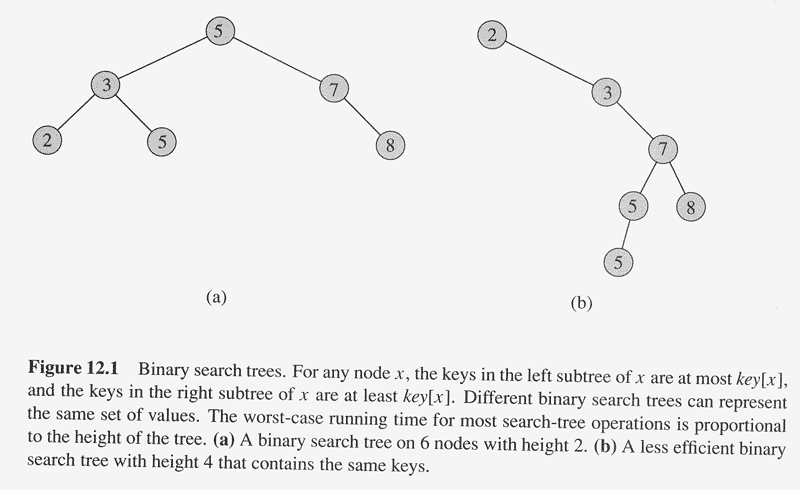
\includegraphics[height=6.5cm]{12-binary-serach-trees.png}
  \end{block}
\end{frame}

\subsection{Inorder Tree Walk}
\begin{frame}
\frametitle{Inorder tree walk}
    Elements are printed in monotonically increasing order.
    How \textsc{Inorder-Tree-Walk} works:
  \begin{itemize}
    \item Check to make sure that $x$ is not NIL.
    \item Recursively, print the keys of the nodes in $x$'s left subtree.
    \item Print $x$'s key.
    \item Recursively, print the keys of the nodes in $x$'s right subtree.
  \end{itemize}
  \begin{columns}
  \column{0.7\textwidth}
  \begin{block}{\textsc{Inorder-Tree-Walk}}
    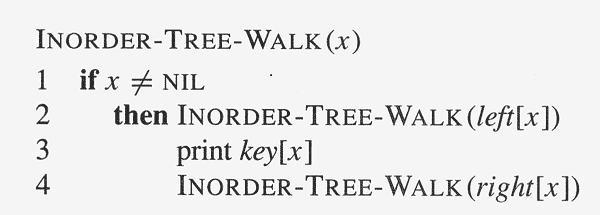
\includegraphics[height=2.7cm]{12-inorder_tree_walk}
  \end{block}

  \column{0.3\textwidth}
  \begin{block}{}
  {\bf\em Time:} Intuitively, the walk takes $\Theta(n)$ time for a tree with $n$ nodes, because we
visit and print each node once.
  \end{block}
  \end{columns}
\end{frame}

\section{Querying A Binary Search Tree}
\subsection{Searching}
\begin{frame}
\frametitle{Searching}
  \begin{block}{\textsc{Tree-Search}}
    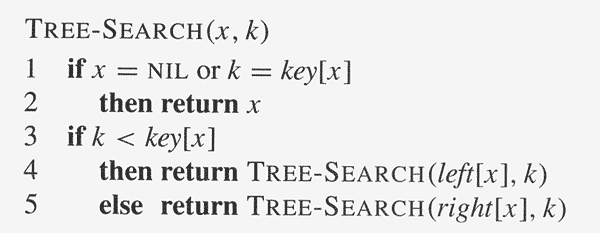
\includegraphics[height=4cm]{12-tree_search}
  \end{block}

  \begin{block}{}
  {\bf\em Time:} The algorithm recurses, visiting nodes on a downward path from the root.
Thus, running time is $O(h)$, where h is the height of the tree.
  \end{block}
\end{frame}

\subsection{Minimum and Maximum}
\begin{frame}
\frametitle{Minimum and maximum}
  The binary-search-tree property guarantees that:
  \begin{itemize}
    \item the minimum key is located at the {\bf \em leftmost} node, and
    \item the maximum key is located at the {bf \em rightmost} node.
  \end{itemize}
  \begin{columns}
  \column{0.4\textwidth}
  \begin{block}{\scriptsize \textsc{Tree-Minimum}}
    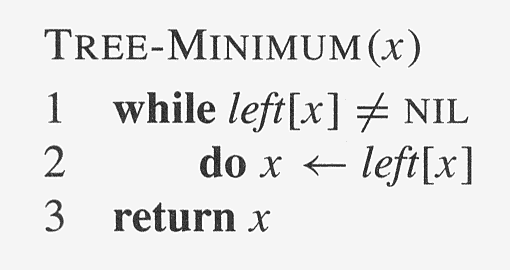
\includegraphics[height=2cm]{12-tree_minimum}
  \end{block}

  \column{0.4\textwidth}
  \begin{block}{\scriptsize \textsc{Tree-Maximum}}
    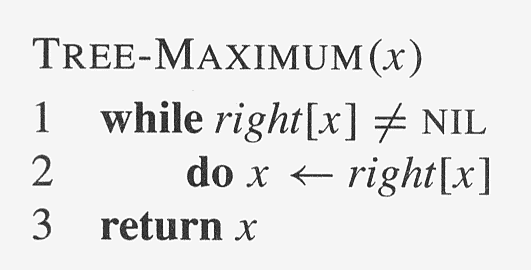
\includegraphics[height=2cm]{12-tree_maximum}
  \end{block}

  \end{columns}
  \begin{block}{}
  {\bf\em Time:} Both procedures visit nodes that form a downward path from the root to a
leaf. Both procedures run in $O(h)$ time, where $h$ is the height of the tree.
  \end{block}
\end{frame}

\subsection{Successor and predecessor}
\begin{frame}
\frametitle{Successor and predecessor}
  {\small The successor of a node $x$ is the node $y$ such that $key[y]$ is the smallest \mbox{key $ > key[x]$}.
  (We can find $x$'s successor based
entirely on the tree structure. No key comparisons are necessary.) If $x$ has the
largest key, then $x$'s successor is NIL.}
  \begin{block}{}
    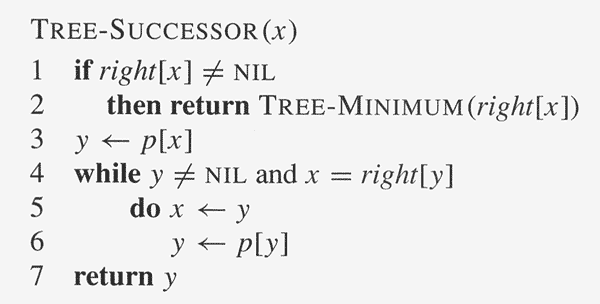
\includegraphics[height=3.5cm]{12-tree_successor}
  \end{block}

  \begin{block}{}
  \small {\bf\em Time:} Since we visit nodes on a path down the tree or up the tree, the running
time is $O(h)$, where $h$ is the height of the tree.
  \end{block}
\end{frame}

\section{Insertion and Deletion}
\subsection{Insertion}
\begin{frame}
\frametitle{Insertion}
  \begin{columns}
  \column[c]{0.8\textwidth}
  \begin{block}{}
    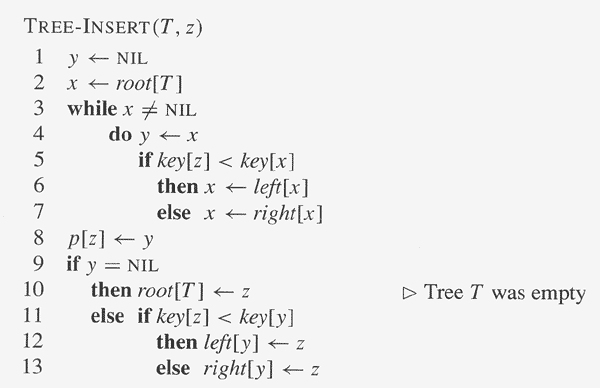
\includegraphics[height=5cm]{12-tree_insert}
  \end{block}
  \end{columns}

  \begin{columns}
  \column[c]{0.8\textwidth}
  \begin{block}{}
    {\small {\bf\em Time:} Same as \textsc{Tree-Search}. On a tree of height $h$, procedure takes $O(h)$ time.}
  \end{block}
  \end{columns}
\end{frame}

%\begin{frame}
%
%\end{frame}

\subsection{Deletion}
\begin{frame}
  \frametitle{Deletion}
  \textsc{Tree-Delete} is broken into three cases. \\
  {\bf \em Case 1:} $z$ has no children.
  \begin{itemize}
    \item Delete $z$ by making the parent of $z$ point to NIL, instead of to $z$.
  \end{itemize}
  {\bf \em Case 2:} $z$ has one child.
  \begin{itemize}
    \item Delete $z$ by making the parent of $z$ point to $z$'s child, instead of to $z$.
  \end{itemize}
  {\bf \em Case 3:} $z$ has two children.
  \begin{itemize}
    \item $z$'s successor $y$ has either no children or one child. ($y$ is the minimum
node---with no left child---in $z$'s right subtree.)
    \item Delete $y$ from the tree (via Case 1 or 2).
    \item Replace $z$'s key and satellite data with $y$'s.
  \end{itemize}
\end{frame}

\begin{frame}
  \begin{columns}
  \column{0.8\textwidth}
  \begin{block}{}
    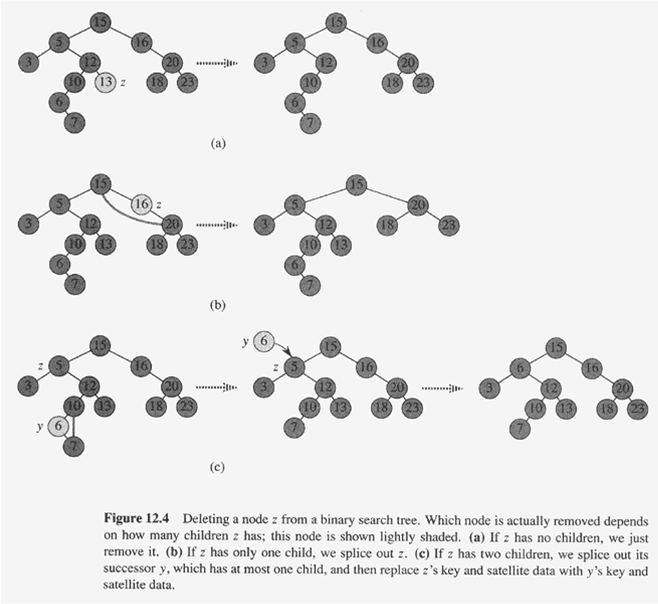
\includegraphics[height=7.2cm]{12-fig-tree_delete}
  \end{block}
  \column{0.2\textwidth}
  \begin{block}{}
    {\small {\bf\em Time:} $O(h)$, on a tree of height $h$.}
  \end{block}
  \end{columns}
\end{frame}

\section{Minimizing Running Time}
\begin{frame}
  \frametitle{Minimizing running time}
  We've been analyzing running time in terms of $h$ (the height of the binary search tree), instead of $n$ (the number of nodes in
the tree).
  \begin{itemize}
    \item {\bf \em Problem:} Worst case for binary search tree is $\Theta(n)$---no better than linked
list.
    \item {\bf \em Solution:} Guarantee small height (balanced tree)---$h = O(\text{lg} n)$.\\
    In later chapters, by varying the properties of binary search trees, we will be
    able to analyze running time in terms of $n$.
    \item {\bf \em Method:} Restructure the tree if necessary.  Nothing special is required for
querying, but there may be extra work when changing the structure of the tree
(inserting or deleting).
  \end{itemize}
\end{frame}
\end{document}
